\begin{figure}[ht]
    \centering
    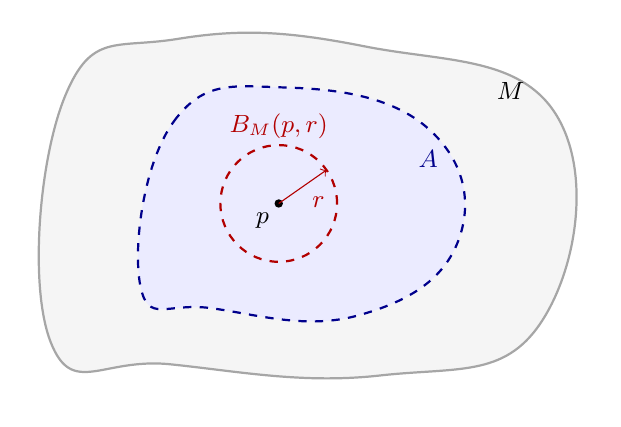
\begin{tikzpicture}[scale=0.95, every node/.style={font=\small}]
        % Espaço ambiente M
        \fill[gray!8]
            plot[smooth cycle, tension=0.75] coordinates {
                (-3.4,-1.8) (-3.2,1.5) (-1.7,2.25) (0.8,2.15)
                (3.35,1.25) (3.15,-1.55) (1.0,-2.25) (-1.8,-2.1)
            };
        \draw[gray!70, thick]
            plot[smooth cycle, tension=0.75] coordinates {
                (-3.4,-1.8) (-3.2,1.5) (-1.7,2.25) (0.8,2.15)
                (3.35,1.25) (3.15,-1.55) (1.0,-2.25) (-1.8,-2.1)
            };
        \node at (2.75,1.55) {$M$};

        % Aberto A
        \fill[blue!8]
            plot[smooth cycle, tension=0.75] coordinates {
                (-2.2,-1.05) (-1.75,1.15) (-0.25,1.6) (1.65,1.05)
                (2.05,-0.45) (0.7,-1.45) (-1.25,-1.35)
            };
        \draw[blue!55!black, thick, dashed]
            plot[smooth cycle, tension=0.75] coordinates {
                (-2.2,-1.05) (-1.75,1.15) (-0.25,1.6) (1.65,1.05)
                (2.05,-0.45) (0.7,-1.45) (-1.25,-1.35)
            };
        \node[blue!55!black] at (1.65,0.65) {$A$};

        % Ponto p
        \coordinate (p) at (-0.35,0.05);
        \fill (p) circle (1.6pt);
        \node[below left] at (p) {$p$};

        % Bola em torno de p contida em A
        \draw[red!70!black, thick, dashed] (p) circle (0.78);
        \node[red!70!black] at (-0.35,1.08) {$B_M(p,r)$};

        % Raio
        \draw[red!70!black, ->] (p) -- ++(35:0.78)
            node[midway, below right] {$r$};
    \end{tikzpicture}
    \caption{Como $A$ é aberto, dado $p\in A$, existe $r>0$ tal que $B_M(p,r)\subseteq A$.}
    \label{fig:restricaoAberto}
\end{figure}
